\section{背景与动机}\label{sec:motivation}

\subsection{LLM 推理及其关键约束}

\begin{figure}[t!]
    \centering
    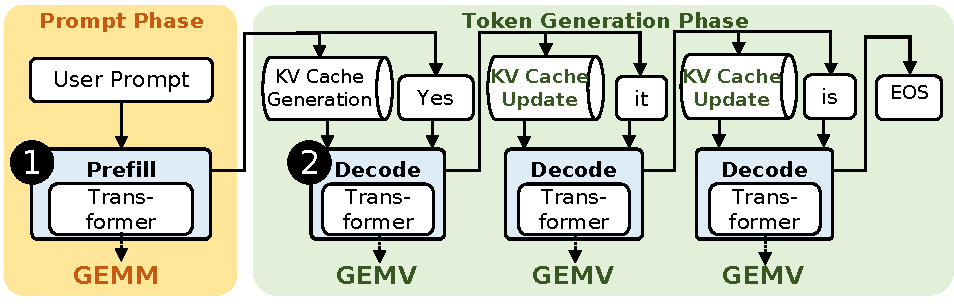
\includegraphics[width=1\linewidth]{imgs/General-LLM.pdf}
    \vspace{-0.3cm}
    \caption{LLM 推理的关键组成部分}
    \label{fig:llm-inference-overview}
    \vspace{-0.3cm}
\end{figure}

如图~\ref{fig:llm-inference-overview} 所示，LLM 推理系统通常以自回归方式逐 token 生成。模型由多个 Transformer 层组成，其中主要是自注意力与前馈模块。推理分为预填充和解码两个阶段：预填充阶段的总周期主要由 GEMM 运算主导（\circled{1}）；解码阶段的总周期则主要由 GEMV 运算主导（\circled{2}）。

LLM 推理受限于内存带宽。模型权重（10--1,000GB）在推理期间要反复从外部内存取入，因为 GPU 通常只有约 100MB 片上内存。对于单个请求，要达到每秒生成数千 token，需要数百 TB/s 带宽，远超当前 GPU 上 HBM（高带宽内存）的能力。

尽管跨 GPU 的张量并行可以增加带宽，但在大型 GPU 集群中缓解通信瓶颈依然困难。增加 GPU 还能提高并发查询的吞吐量，却不能降低单个输出 token 的时间（TPOT），因为每个查询仍受内存带宽限制。

\vspace{-3mm}
\subsection{采用晶圆级加速器的原因}
\vspace{-1mm}

\begin{table}[t]
\resizebox{\linewidth}{!}{%
\begin{tabular}{|c|c|c|}
\hline
 & 裸片级系统 & 晶圆级系统 \\ \hline
面积（mm$^2$） & 最高 858 & 最高 73062 \\ \hline
晶体管数（TSMC n3） & 约 1 万亿 & 约数十万亿 \\ \hline
核心数 & 数千--数万 & 十万--百万 \\ \hline
片上内存 & 数十--数百 MB & 约数十 GB \\ \hline
内存带宽 & 数 TB/s & 约数十 PB/s \\ \hline
连接的 HBM & 约数十--数百 GB & 数十 TB（通过 TSMC SoW）\cite{tsmc-advanced-packaging} \\ \hline
\begin{tabular}[c]{@{}c@{}}裸片间带宽\\（TB/s）\end{tabular} & 约 1--10（片外） & 约 10--100（片上） \\ \hline
\begin{tabular}[c]{@{}c@{}}裸片间延迟\\（ns）\end{tabular} & 约数百（片外） & 约个位数（片上） \\ \hline
\begin{tabular}[c]{@{}c@{}}裸片间能耗\\（pJ/bit）\end{tabular} & 约数十（片外） & 约零点几（片上） \\ \hline
\end{tabular}%
}
    \vspace{-2mm}
\caption{裸片级系统与晶圆级系统的比较}
    \vspace{-3mm}
\label{tab1:die-scale-vs-wafer-scale}
\end{table}

为了提高内存带宽，加速器设计者出于以下原因正越来越多地采用晶圆级系统集成~\cite{tsmc-advanced-packaging}：

\mypar{性能优势} 如表~\ref{tab1:die-scale-vs-wafer-scale} 所示，晶圆级系统技术允许在单颗晶圆级芯片中集成数万亿晶体管，最多是典型 GPU 裸片的 $100\times$。因此可以集成数百万个面向 AI 优化的核心，提供数十 GB 片上内存和最高数十 PB/s 内存带宽，后者是标准 GPU 数 TB/s 带宽的 $1{,}000\times$。与标准裸片相比，未来的晶圆级芯片还可在边缘连接多 $40$--$80\times$ 的 HBM 芯片~\cite{tsmc-advanced-packaging}。

\mypar{集成效率} 晶圆级系统擅长集成海量并行核心。与传统基于 PCB 的芯片间互连（例如 NVIDIA NVLink、PCIe）相比，晶圆上的裸片间连接可在单位面积上提供最高 $10\times$ 带宽、$100$--$300\times$ 的延迟优势，以及每 bit 近 $100\times$ 的能效提升~\cite{wse}，如表~\ref{tab1:die-scale-vs-wafer-scale} 所示。前文已经指出，LLM 推理因密集数据访问而主要受内存带宽约束。在分布式环境中，远程内存访问引起的芯片间通信开销会限制扩展性，解码阶段的 GEMV 尤其如此。因此，与传统芯片间链路相比，晶圆级系统集成能提供延迟更低、带宽更高的互连，并改善效率。

\mypar{更低成本} 晶圆级集成可以降低制造成本，因为制造成本中相当大的一部分（通常为 30--50\%）来自对单颗芯片的测试与封装~\cite{wiki:waferscale}。此外，晶圆级集成在提升良率方面已取得显著进展。台积电等公司也在开发把经过完整测试的裸片集成到同一晶圆上的技术，以进一步改善良率。

\vspace{-3mm}
\subsection{晶圆级 LLM 推理面临的挑战}
\vspace{-1mm}

利用晶圆级加速器进行 LLM 推理的核心挑战，在于它们在单颗芯片上转向了分布式、非均匀内存架构。如图~\ref{fig:mesh-architecture}(a) 所示，现有 LLM 系统针对共享内存（单芯片）或全互连架构（例如 GPU pod）进行了优化。然而，随着片上内存容量增长，这些架构面临指数增长的制造成本和性能下降，因而必须采用分布式片上架构。

如图~\ref{fig:mesh-architecture}(b) 所示，AI 加速器设计者主要使用\textbf{类网格片上网络（NoC）}连接\textbf{海量核心}（从数十万到数百万）。网格拓扑有利于高效排列核心，并能有效解决散热~\cite{cooling}、供电~\cite{powerdelivery}和低成本布线~\cite{chip-cost-1,chip-cost-2}问题；每个核心只与附近邻居通信，如图~\ref{fig:mesh-architecture}(b) 所示。3D 环面或树结构等其他拓扑因片上布线成本过高而不切实际。因此，Cerebras WSE~\cite{wse} 和 Tesla Dojo~\cite{dojo} 等晶圆级芯片厂商均采用超大规模网格架构。即使是 Meta MTIA~\cite{mtia}、Tenstorrent~\cite{tenstorrent} 等非晶圆级加速器~\cite{amd-xdna,azure-maia}，也使用网格来扩展单芯片内的核心数量。

\begin{figure}[t]
    \centering
    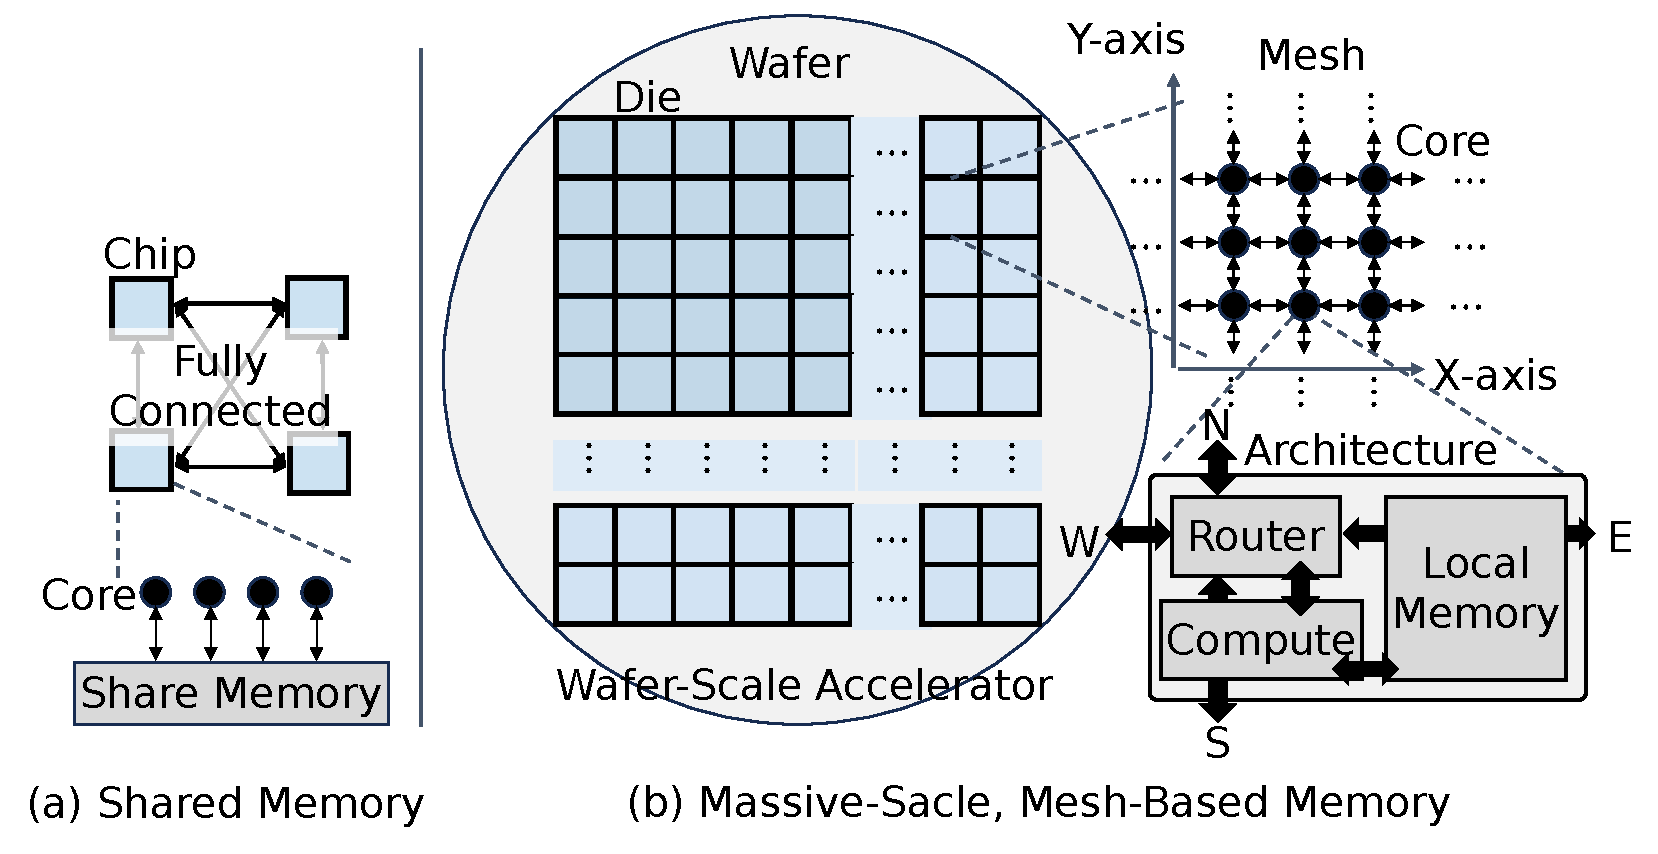
\includegraphics[width=1\linewidth]{imgs/die_on_wafer.pdf}
    \vspace{-3mm}
    \caption{超大规模、基于网格的内存架构}
    \vspace{-3mm}
    \label{fig:mesh-architecture}
\end{figure}

超大规模网格架构给多种 LLM 运算带来挑战，因为它们需要大量数据移动：（i）管理 LLM 模型与 KV cache；（ii）预填充阶段的 GEMM 运算；（iii）解码阶段的 GEMV 运算。点积和激活函数等逐元素运算不需要移动数据，天然受益于并行。RMSNorm 和 Softmax 等需要 allreduce 的运算，则可以复用 GEMV 方案。
